\section{Proposed Work}

{The bulk of work between this proposal and the dissertation defense would focus on bringing together the four aforementioned themes. Work would consist of three main trajectories: (i) the development of \textbf{CityScopeJS}, a unified CityScope interface for interaction, analysis, and intervention, (ii) further development of \textbf{CityIO}, a backend system for distributed urban analytics modules, and (iii) deployment and integration of CityScope in additional real-world use cases (Hamburg, Vietnam, Andorra, South America, etc).}

\begin{figure}[t]
\begin{center}
    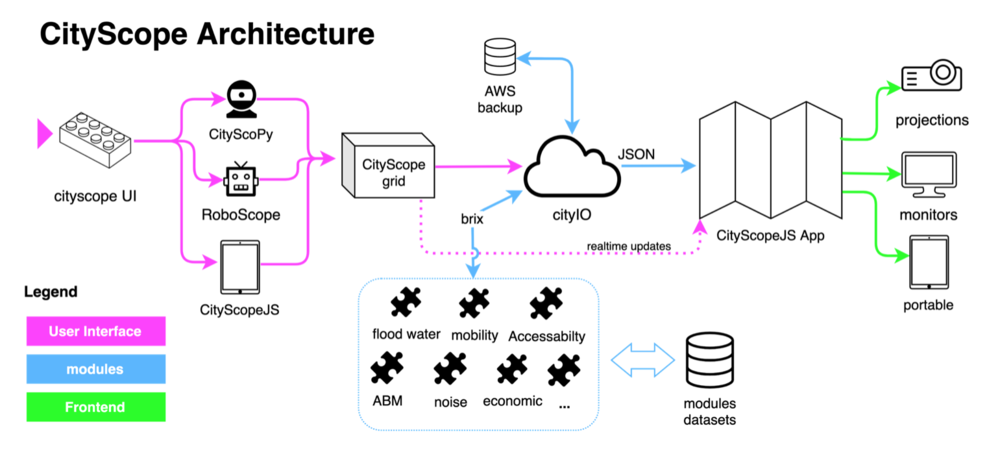
\includegraphics[width=0.8\textwidth]{figures/csjs_arch.png}
\end{center}
   \caption{CityScopeJS and the new CityScope Architecture. This diagram presents the data flow and different components of the current CityScope architecture: (left) different modules control the inputs and grid interaction. (center) upon interaction, cityIO VPC handles the transaction with different urban analytics modules. (right) When these computation phase is complete, the grid and analysis modules results are sent to output devices, either online (CityScopeJS, API), or physical (projectors, monitors)}
\label{fig:csjs_arch}
\end{figure}


{\textbf{CityScopeJS}: A unified interface for the CityScope platform is the \textbf{CityScopeJS} (2018-current) project. This flavor of CityScope attempts to combine many of the aspects of prior tools in one comprehensive and reusable system. In \textbf{CityScope Grasbrook} (2018-2020) and \textbf{CityScope Corktown} (2019-2020) the goal of simulating planning and mobility scenarios was achieved by incorporating interactive, real-time, and collaborative urban planning processes in one web-based, TUI-enabled, modular system.}

\begin{figure}[t]
\begin{center}
    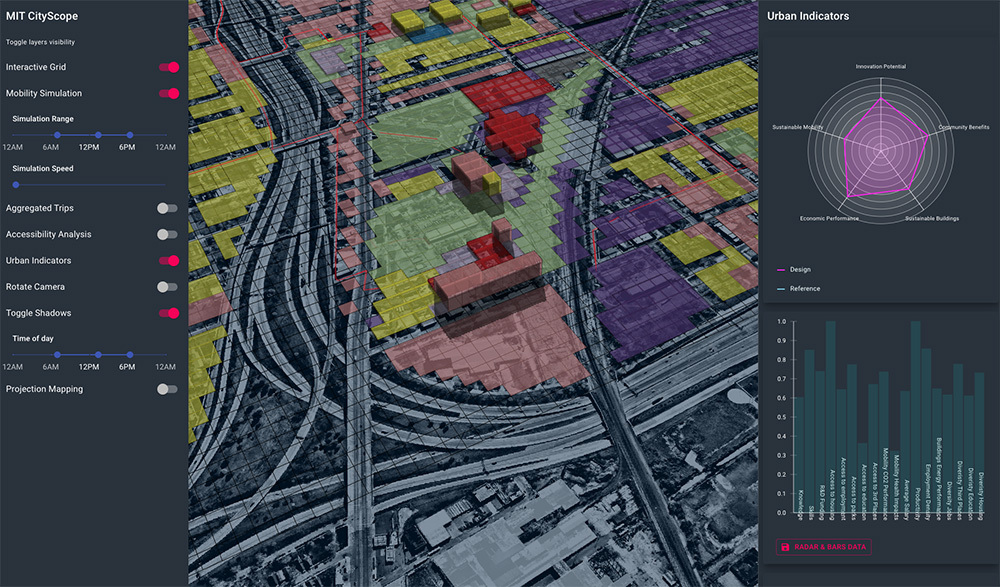
\includegraphics[width=1\textwidth]{figures/csjs.jpg}
\end{center}
   \caption{CityScopeJS interface. As with the TUI versions of CityScope, users interact with a simple, geo-located grid. Interactions are sent to the cityIO analysis modules, and their responses are then displayed spatially as heat-maps, trips, or graphically as charts and data visualisations. The same interface can then be also used with tangible interfaces, robotic UIs, AR or VR.}
\label{fig:csjs}
\end{figure}

{\textbf{CityScope Modules}: At the backend of CityScope, there are growing number of analysis modules design to react in real-time to user interaction. These modules can be global (such as density or shade analysis) or project-site specific (such as accessibility, mobility, storm-water or noise). CityScope is designed to allow both classes of modules to be adapted to most instances of the system. The dissertation will expand on the architecture of the system, its pros and cons, and future prospects.}


{\textbf{Deployments}:The thesis will explore in-progress and future development and implementation of CityScope in Hamburg, Vietnam, Guadalajara, Andorra, as well as other use-cases as they emerge.}


\subsection{Timeline}

\begin{itemize}
\item {2021 - early 2022 -- Finalize new CityScope Architecture development, deployment, and documentation. The goal is to stabilize open-source development efforts of the platform's different components (input - modules/cityIO - UI/output) to allow streamlined deployment for upcoming CS projects.}
	
\item CityScope Corktown: document and submit publication for the CityScope project in Detroit, MI. 

\item {CityScope Grasbrook: complete development and submit publication for the CityScope project in Grasbrook, Hamburg, DE.}
	
\item {Andorra Mobility during COVID-19: Analyze the relationship between COVID-19 spread and the country's mobility pattern retrieved from high-res telecom data. Will complete publication and submit to high-quality venue.}
	
\item {MITOS: Conduct research, development, and deployment of MIT Sustainability Office CityScope project. Investigate impacts of new campus mobility policies in response to COVID-19. Propose feasible interventions via a dynamic CS interface.}  
	
\item {RoboScope: support the development and deploy CityScope robotic interface to the CityScope Volpe platform using CSjs modules.}

\item May 2021 -- Writing. 
\item Feb 2022 -- Defense.
\item April 2022 -- Final changes and submission. 
\end{itemize}